\documentclass{standalone}

\usepackage{tikz}
\usetikzlibrary{calc,trees,positioning,arrows,fit,shapes,calc}
\begin{document}
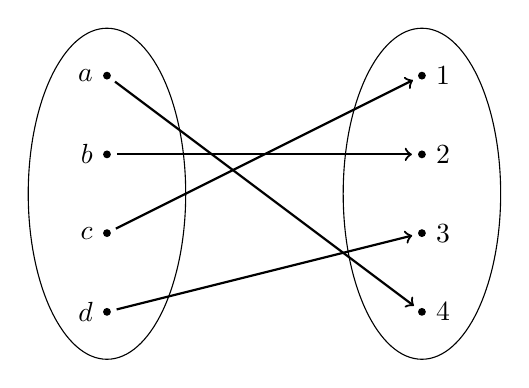
\begin{tikzpicture}[ele/.style={fill=black,circle,minimum width=.8pt,inner sep=1pt},every fit/.style={ellipse,draw,inner sep=-2pt}]
      \node[ele,label=left:$a$] (a1) at (0,4) {};    
      \node[ele,label=left:$b$] (a2) at (0,3) {};    
      \node[ele,label=left:$c$] (a3) at (0,2) {};
      \node[ele,label=left:$d$] (a4) at (0,1) {};
    
      \node[ele,,label=right:$1$] (b1) at (4,4) {};
      \node[ele,,label=right:$2$] (b2) at (4,3) {};
      \node[ele,,label=right:$3$] (b3) at (4,2) {};
      \node[ele,,label=right:$4$] (b4) at (4,1) {};
    
      \node[draw,fit= (a1) (a2) (a3) (a4),minimum width=2cm] {} ;
      \node[draw,fit= (b1) (b2) (b3) (b4),minimum width=2cm] {} ;  
      \draw[->,thick,shorten <=2pt,shorten >=2pt] (a1) -- (b4);
      \draw[->,thick,shorten <=2pt,shorten >=2] (a2) -- (b2);
      \draw[->,thick,shorten <=2pt,shorten >=2] (a3) -- (b1);
      \draw[->,thick,shorten <=2pt,shorten >=2] (a4) -- (b3);
     \end{tikzpicture}
\end{document}